%\documentclass[journal]{IEEEtran}
\documentclass[8pt]{article}

\usepackage{amsmath,amssymb,caption,comment,enumitem,float,graphicx,microtype}
\usepackage[utf8]{inputenc}
\usepackage[T1]{fontenc}
\usepackage[margin=1in]{geometry}
\usepackage{setspace}
\usepackage{fancyhdr}
\usepackage{bm}
\usepackage{caption}
\usepackage{subcaption}
\pagestyle{fancy}
\fancyhf{}
\rhead{Anonymous Authors \\ \today}

\newcommand{\N}{{\mathbb N}}
\newcommand{\Z}{{\mathbb Z}}
\newcommand{\Q}{{\mathbb Q}}
\newcommand{\R}{{\mathbb R}}
\newcommand{\C}{{\mathbb C}}
\newcommand{\F}{{\mathbb F}}
\newcommand{\E}{{\mathbb E}}
\mathchardef\hyphen="2D

\title{\vspace{-5ex} 6.867 Homework 1}
\author{}
\date{\vspace{-9ex}}

\begin{document}

\maketitle
\thispagestyle{fancy}

%#############################
%TODO: 1. Check tense so it's consistent

%-------------------------------------------
%===============SECTION ONE=================
%-------------------------------------------

\section{Implementing Gradient Descent}

In any gradient descent algorithm, the main hyperparameters we have to tune are the initial point we start the gradient descent from, the step size, and the convergence criteria. 
%
%\begin{itemize}
%
%\item An incorrect initial guess could lead to getting stuck at a local min without ever reaching the global minumum
%\item A step size that is too large can shoot past the minumum or go back and forth without ever reaching the critical point. Conversely, a step size that is too small can make the algorithm take far too long to converge.
%\item A convergence criteria that is too lax can result in a sub-optimal stopping point, while a convergence criteria that is too strict can result in the algorithm taking too long.
%
%\end{itemize}

For each of the three parameters, we can see how varying the parameters changes the gradient descent for both of the provided functions (the Gaussian and the bowl).

Unless otherwise specified, default parameters are: starting point = (0,0), step size = 0.01, and convergence criteria of difference between consecutive objective function values is less than $10^{-10}$.
%
\begin{figure}[H]
\centering
        \begin{subfigure}[b]{0.38\textwidth}
                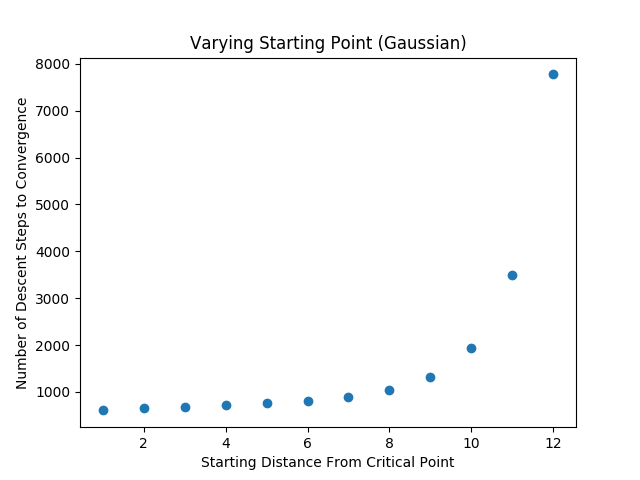
\includegraphics[width=\linewidth]{../P1/figs/start_gauss.png}
        \end{subfigure}%
        \begin{subfigure}[b]{0.38\textwidth}
                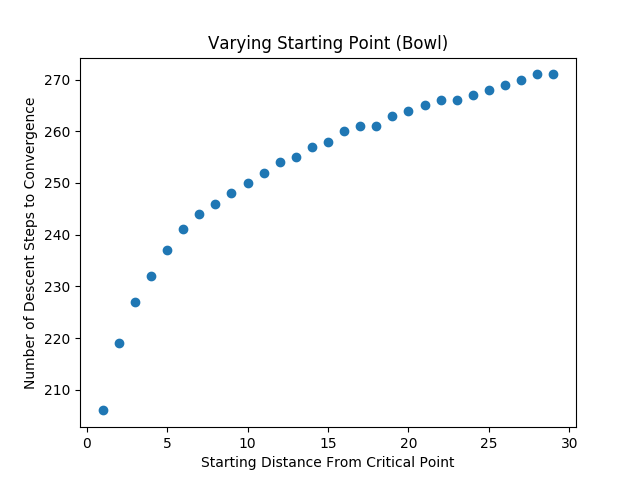
\includegraphics[width=\linewidth]{../P1/figs/start_bowl.png}
        \end{subfigure}%
\end{figure}
%
The number of steps needed for convergence grows much faster in the Gaussian than it does with the bowl. This is because the gradient decays exponentially in the Gaussian case with respect to distance from the critical point but linearly in the bowl case.
%
\begin{figure}[H]
\centering
        \begin{subfigure}[b]{0.38\textwidth}
                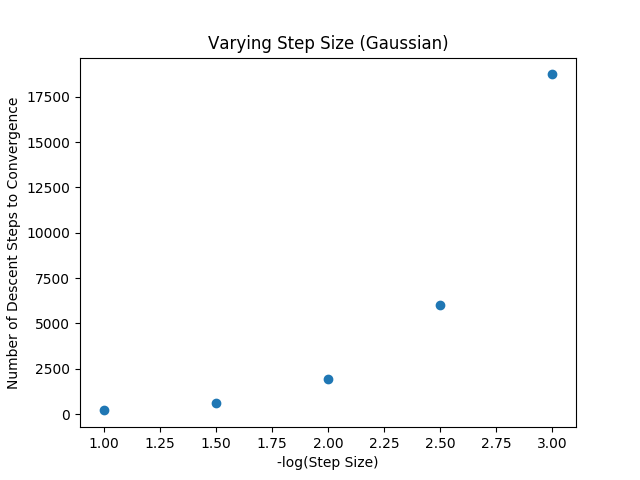
\includegraphics[width=\linewidth]{../P1/figs/step_gauss.png}
        \end{subfigure}%
        \begin{subfigure}[b]{0.38\textwidth}
                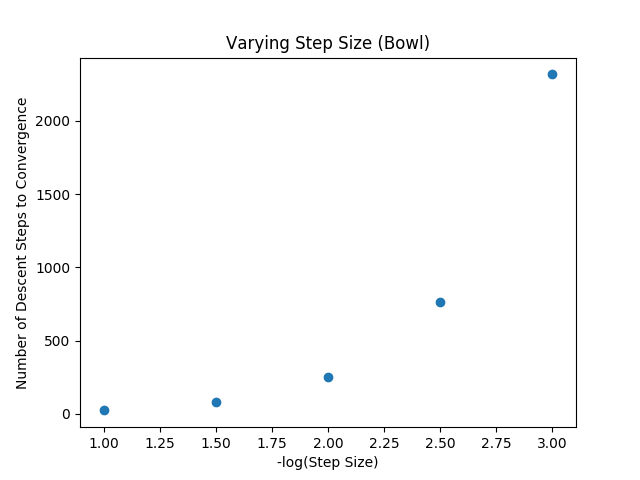
\includegraphics[width=\linewidth]{../P1/figs/step_bowl.png}
        \end{subfigure}%
\end{figure}
%
In both cases, step size eventually grows linearly with the number of steps needed until convergence. However, in some cases where the step size is extremely large (not shown), the function may not converge at all.
%
\begin{figure}[H]
\centering
        \begin{subfigure}[b]{0.38\textwidth}
                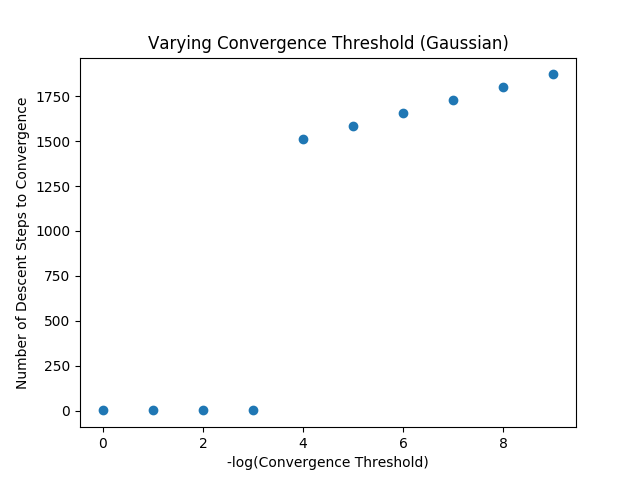
\includegraphics[width=\linewidth]{../P1/figs/converge_gauss.png}
        \end{subfigure}%
        \begin{subfigure}[b]{0.38\textwidth}
                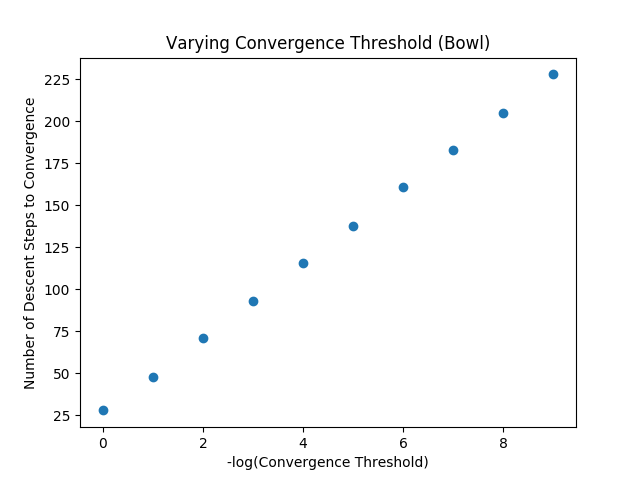
\includegraphics[width=\linewidth]{../P1/figs/converge_bowl.png}
        \end{subfigure}%
\end{figure}
%
Here, as the convergence threshold grows, so to does the number of steps needed to converge. Intuitively, this makes sense--the more accurate the gradient descent needs to be, the more iterations we need to converge.
%
\begin{figure}[H]
\centering
        \begin{subfigure}[b]{0.4\textwidth}
                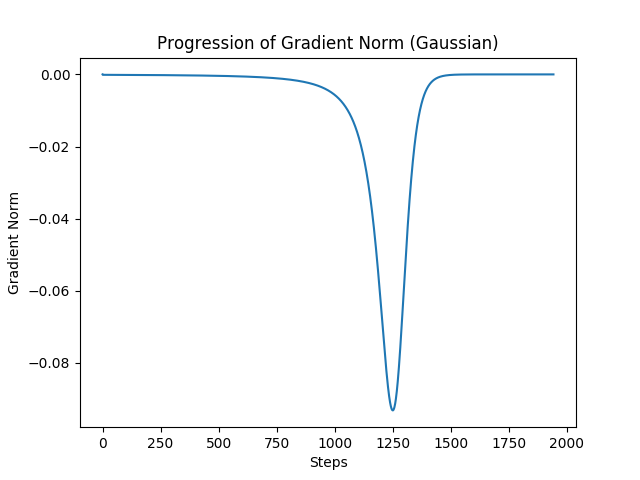
\includegraphics[width=\linewidth]{../P1/figs/grad_norm_gauss.png}
        \end{subfigure}%
        \begin{subfigure}[b]{0.4\textwidth}
                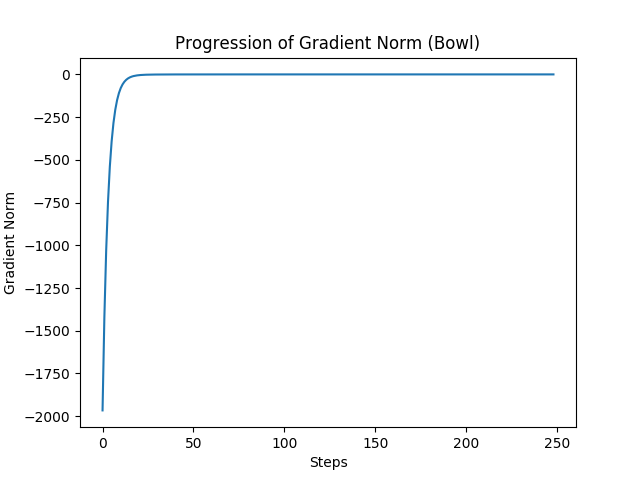
\includegraphics[width=\linewidth]{../P1/figs/grad_norm_bowl.png}
        \end{subfigure}%
\caption*{As mentioned before, the gradient norm of the Gaussian starts off very small when the starting point is far away from the critical point. Around step 1000, it starts to reach the steep part of the Gaussian, at which point it quickly reaches convergence. For the bowl, the gradient norm starts off high and quickly decreases and converges.}
\end{figure}

To perform gradient descent on functions that do not have a clean, closed-form gradient, we can approximate the gradient using central differences. Here, we analyze how the performance of the central differences approximation varies based on the step size used for the difference approximation.

\begin{figure}[H]
\centering
        \begin{subfigure}[b]{0.4\textwidth}
                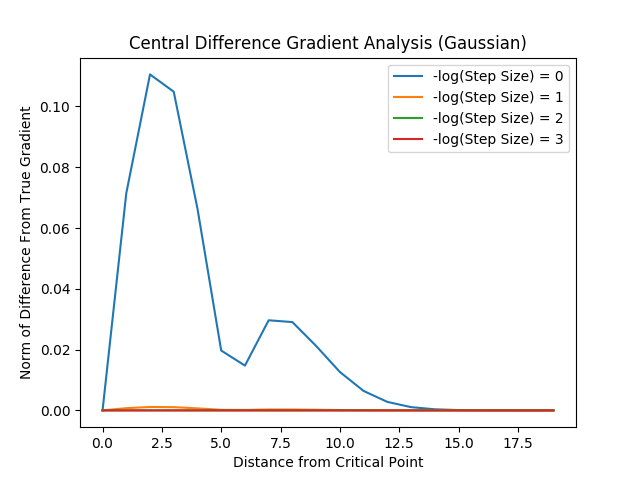
\includegraphics[width=\linewidth]{../P1/figs/central_diff_gauss.png}
        \end{subfigure}%
        \begin{subfigure}[b]{0.4\textwidth}
                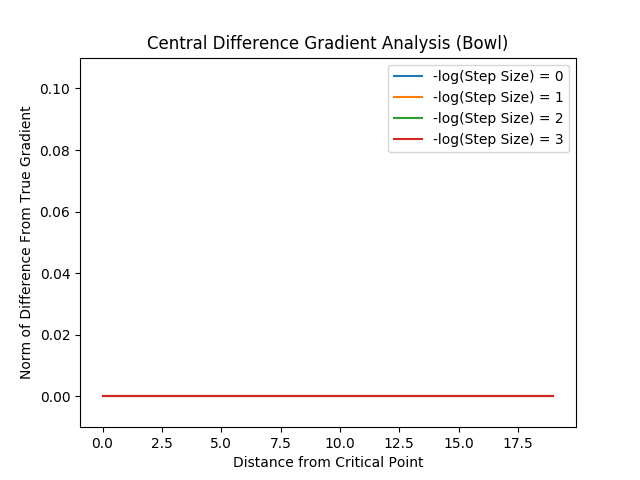
\includegraphics[width=\linewidth]{../P1/figs/central_diff_bowl.png}
        \end{subfigure}%
\caption*{When the step size is larger than $10^{-2}$, we start to see errors in the Gaussian. For the bowl, we have no error in our gradient approximation regardless of step size because the gradient of the bowl is linear; because of this, our averaging approximation acutally gives us the exact answer. }
\end{figure}

Often, when running gradient descent, it is computationally expensive to calculate the total error. We can use Stochastic Gradient Descent as an alternative: each time we calculate the least square error, we only use one sample to calculate the error. This results in a much faster overall computation at the expense of some accuracy. We can compare the two algorithms by calculating the gradient descent of the least square error with similar convergence criteria.

\begin{figure}[H]
\centering
        \begin{subfigure}[b]{0.4\textwidth}
                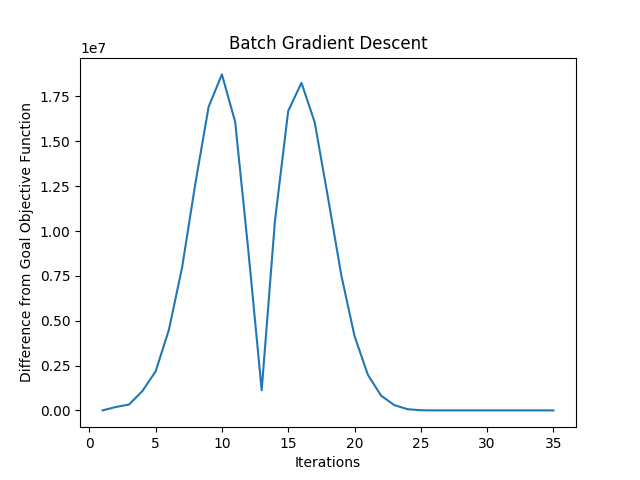
\includegraphics[width=\linewidth]{../P1/figs/plot_batch.png}
        \end{subfigure}%
        \begin{subfigure}[b]{0.4\textwidth}
                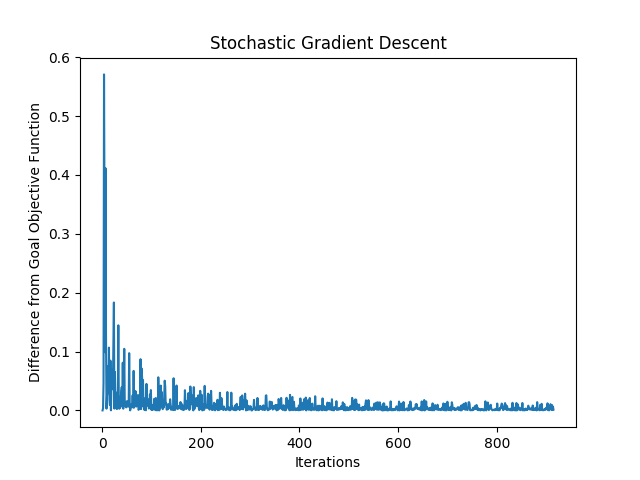
\includegraphics[width=\linewidth]{../P1/figs/plot_sgd.png}
        \end{subfigure}%
\caption*{It takes many more iterations for SGD to converge than batch descent. Furthermore, batch descent can converge on a more accurate answer (due to the randomness of SGD throwing things off). However, SGD runs much faster, even while taking more iterations. In practice, mini-batch SGD is often used as the best of both worlds.}
\end{figure}

%-------------------------------------------
%===============SECTION TWO=================
%-------------------------------------------

\section{Linear Basis Function Regression}

%---------------Section 2.1-----------------
\subsection{Closed-form Solution with Polynomial Basis}
% Replicate plots
Consider the basis function $$\bm \Phi_M(x) = [\phi_0(x), \dots, \phi_M(x)],$$ where each $\phi_k(x) = x^k$. Applying $\bm \Phi_M$ to $\mathbf{X}$ gives the desired basis change, so we have the generalized linear model
\[
\mathbf Y = \bm \Phi_M(\mathbf X) \cdot \bm \theta + \bm \epsilon,
\]
which has the close-form solution (from first order conditions on the least squares error\footnotemark),
%
\begin{align*}
\hat{\bm \theta} = (\bm \Phi_M(\mathbf X)^T \bm \Phi_M(\mathbf X))^{-1} \bm \Phi_M(\mathbf X)^T \mathbf Y
\end{align*}
%
where $\hat{\bm \theta}$ is the maximum-likelihood estimator of the regression coefficients.

\footnotetext{See section 2.2 for a derivation of the gradient vector.}

We fit polynomial regressions on the data via this method with a few different max degrees $(M = 0, 1, 3, 10)$. Below are the resulting polynomials, plotted against the original data and source function:%\footnotemark:

% \footnotetext{See the appendix for the numerical coefficients from the regression.}

\begin{figure}[H]
  \centering
  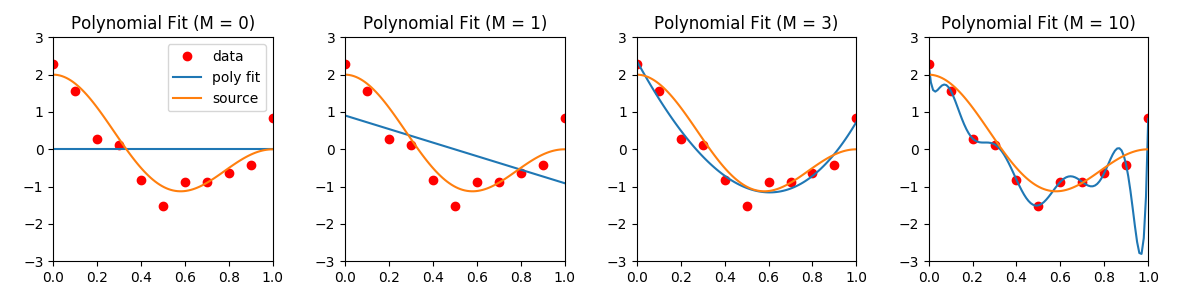
\includegraphics[width = 6.5in]{../P2/figs/part_1.png}
  \caption{M-Degree Polynomial Fit}
\end{figure}

It appears that $M = 3$ gives the closest interpolation of the true function. We infer that $M = 0, 1$ give a poor fit as the models do not have sufficient degrees of freedom, while $M = 10$ has too many paramters and leads to overfitting.

%-------------Section 2.2---------------
\subsection{Closed-form Gradient of Squared Error}

We take a second approach to finding the least squares estimators (which also happen to be maximum likelihood estimators). The residual sum of squares for weight vector $\theta$ is given by
\[
loss(\bm \theta) = |(\bm Y - \bm \Phi_M(\bm X) \bm \theta)|^2.
\]
Differentiating the error function with respect to $\bm \theta$ gives the gradient function
%
 \begin{align*}
   \frac{\partial }{\partial \bm \theta} |(\bm Y - \bm \Phi_M(\bm X) \bm \theta)|^2 &= \frac{\partial }{\partial \bm \theta} [(\bm Y - \bm \Phi_M(\bm X) \bm \theta)^T \cdot (\bm Y - \bm \Phi_M(\bm X) \bm \theta)] \\
   &= \frac{\partial }{\partial \bm \theta} [- (\bm \Phi_M(\bm X) \bm \theta)^T \bm Y - \bm Y^T (\bm \Phi_M(\bm X) \bm \theta) + \bm \theta^T \bm \Phi_M(\bm X)^T \cdot (\bm \Phi_M(\bm X) \bm \theta)] \\
   &= -2  \cdot \bm \Phi_M(\bm X)^T \bm Y + 2 \cdot \bm \Phi_M(\bm X)^T \bm \Phi_M(\bm X) \bm \theta
 \end{align*}
%
Using the numerical derivative code in Section 1, we tested the correctness of the closed-form gradient on a few different $\bm \theta, M$ values, and the results are all accurate within $10^{-10}$ of each other.\footnotemark

\footnotetext{Measured in the squared norm of the difference.}

%-----------Section 2.3-----------------
\subsection{Gradient Descent Solution with Polynomial Basis}
% Minimize SSE with Batch GD and SGD
% smallers thresholds produces slightly better fits when learn rate is small
% any threshold smaller than 1e-6 has similar results for learn rates we tested
% sgd is more sensitive to start point compared to bgd
% learn rate can't be too high or too low: doesn't converge when learn rate is too high, converges immediately when learn rate is too low (and when threshold is not adjusted accordingly)
% sgd is much more sensitive to learn rate as well
% stucks in local minima when degree is high -> more local minima
We run batch and stochastic gradient descent on the square loss, and experimented with differents start points, convergence thresholds, and learning rates (i.e. step sizes). We find that the smaller convergence thresholds produce slightly better fits, which is expected, but the effect is not significant. During our experimentation, convergence thresholds smaller than $10^7$ generally produced the same weights.

We also find higher degree models are more sensitive to the start point than the low degree models. This is likely because models with a higher degree $M$ have more local minima that the algorithm may converge to.

In addition, we find that the solutions are quite sensitive to the learning rates, and that SGD tend to require a higher learning rate than Batch in general to achieve a reasonable fit. Since the gradient vector at each step in SGD much noiser compared to in Batch, SGD has is more likely to descend into some spurious equilibrium. This can be partially compensated by a higher learning rate. (However, a learning rate too large causes the the algorithm to skip over the global minima to fail to converge.)

% TODO: EXPLAIN IN TERMS OF PROPERTIES OF FUNCTION

By similar reasoning, we find that Batch produces a much better fit than SGD, especially given the small data set (so runtime is not an issue). This is illustrated by plots of Batch and SGD below (start point $=\bm 0$, convergence threshold $=10^{-8}$):

\begin{figure}[H]
  \centering
  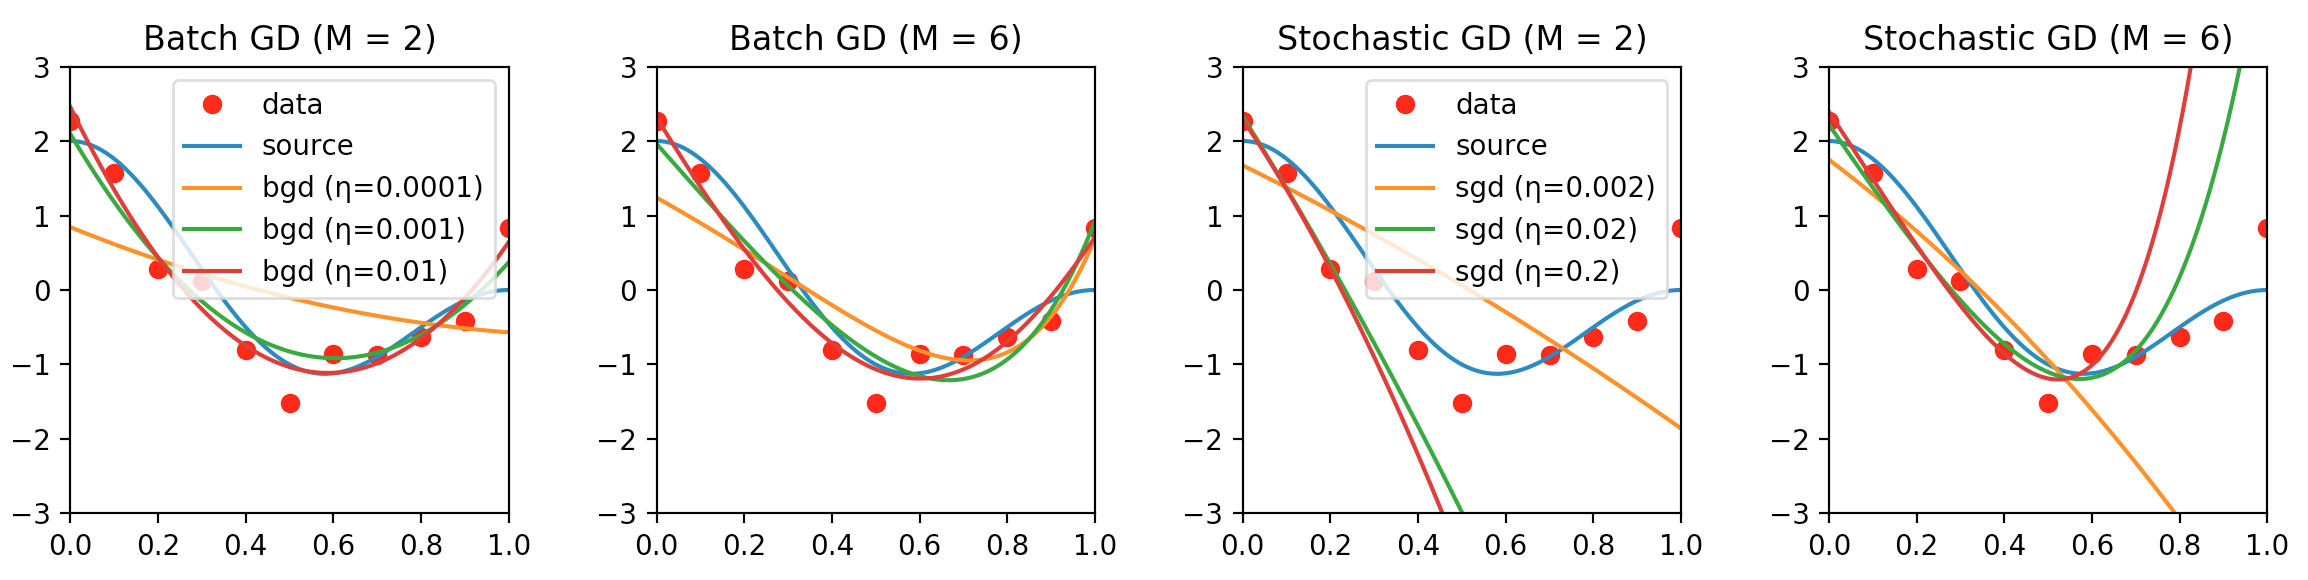
\includegraphics[width = 6.5in]{../P2/figs/part_3.png}
  \caption{Batch and Stochastic Gradient Descent with Various Learning Rates $\eta$}
\end{figure}


%----------Section 2.4------------------
\subsection{Closed-form Solution with Cosine Function Basis}

We apply the same technique as in section 2.1, but now with cosine functions as basis. We apply the basis transformation of degree $M$
$$\bm \Phi_M(x) = [\phi_1(x), \dots, \phi_M(x)],$$ where each $\phi_k(x) = cos(k \pi x)$, and solve for closed-form solutions to the generalized linear model of degrees M = 1, 2, 4, 8. We plot the results against the data and source below:
\begin{figure}[H]
  \centering
  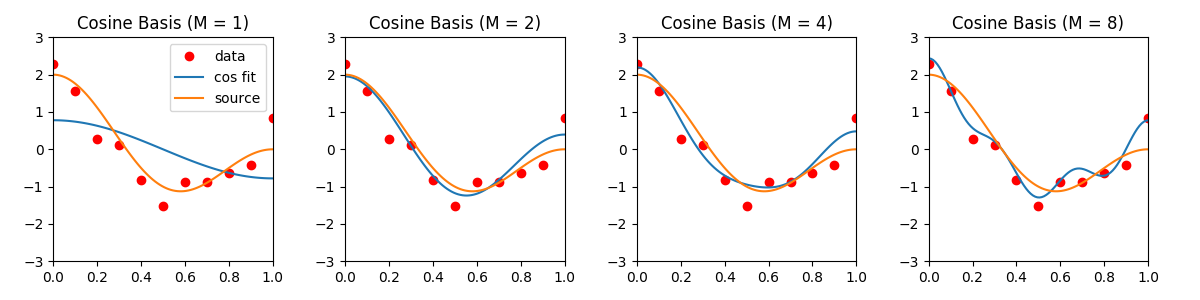
\includegraphics[width = 6.5in]{../P2/figs/part_4.png}
  \caption{Cosine Functions Fit}
\end{figure}
Again, $M = 2$ seems to give the best fit of the true function, and overfitting behavior is clear when the degree is high (such as in $M=8$).

For $M = 2$, the regression result is $f(x) = 0.78 \cos(\pi x) + 1.17 \cos(2\pi x)$, which resembles the true function pretty well for most values of $x$, as seen in the plot. However, the coefficient estimates are still off by around 20\%, which is not surprising given the very limited amount of data.

%-------------------------------------------
%==============SECTION THREE================
%-------------------------------------------

\section{Ridge Regression}

We first run ridge regression on the polynomial basis data set from the previous problem. Given that we are trying to minimize the squared error  $\vert \vert X\theta - y\vert \vert ^2 + \lambda \vert \vert \theta \vert \vert ^2$, the closed form solution gives us:

\[  \theta = (X^{T}X + \lambda I)^{-1} X^{T} y \]

We plot the MSE for different dimensionality models for different values of $\lambda$.
%
\begin{figure}[H]
  \centering
  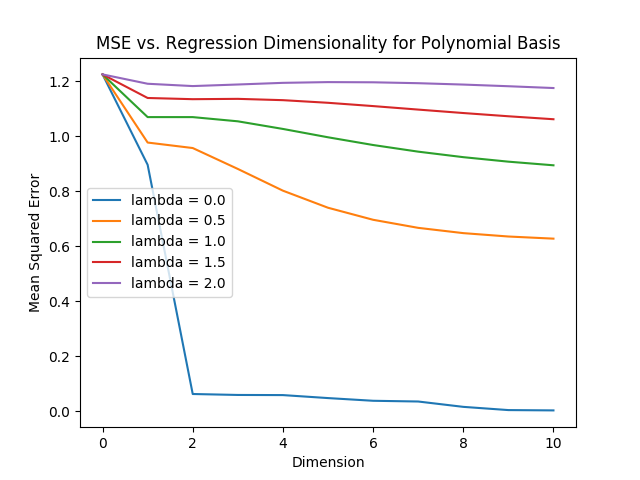
\includegraphics[width = 3.2in]{../P3/figs/poly_basis.png}
  \caption*{For $\lambda = 0$, increasing the dimensionality slowly improves the MSE. However, as $\lambda$ grows, the benefit shrinks because the regularization term punishes large terms in $\theta$.}
\end{figure}
%
We then run our ridge regression on the provided datasets. For each value of $\lambda$, we run ridge regression for different values of M and pick the model with the best validation error. We then run that model on the test set and compute the MSE.
%
\begin{center}
 \begin{tabular}{||c c c c||} 
 \hline
 \multicolumn{4}{|c|}{Train on A, Test on B} \\
 \hline
 \hline
 $\lambda$ & Optimal M & Validation MSE & Test MSE\\ [0.5ex] 
 \hline\hline
 0 & 2 & 0.107 & 2.575 \\ 
 \hline
 0.5 & 2 & 0.126 & 2.566 \\
 \hline
 1 & 2 & 0.147 & 2.564 \\
 \hline
 1.5 & 2 & 0.170 & 2.566 \\
 \hline
2 & 1 & 0.188 & 2.584 \\
 \hline
2.5 & 1 & 0.206 & 2.604 \\
 \hline
3 & 1 & 0.225 & 2.623 \\
 \hline
 3.5 & 1 & 0.245 & 2.643 \\
 \hline
4 & 1 & 0.265 & 2.662 \\
 \hline
\end{tabular}
\end{center}
%
These results look weird because the test errors are so much higher than the validation errors. This is because there is a clear outlier data point in B that throws off the MSE.

\begin{figure}[H]
\centering
        \begin{subfigure}[b]{0.4\textwidth}
                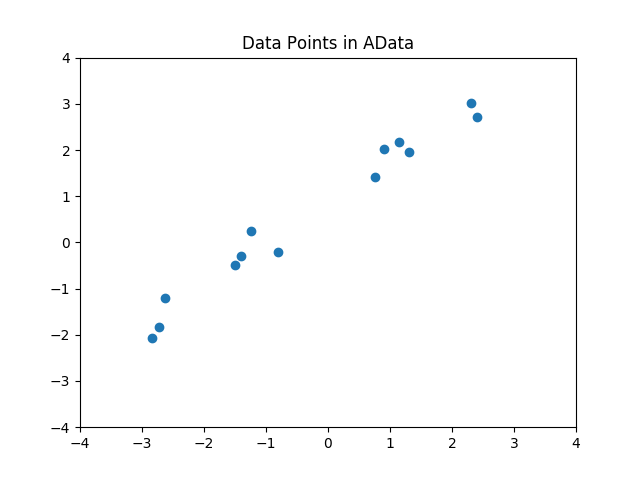
\includegraphics[width=\linewidth]{../P3/figs/A_data.png}
        \end{subfigure}%
        \begin{subfigure}[b]{0.4\textwidth}
                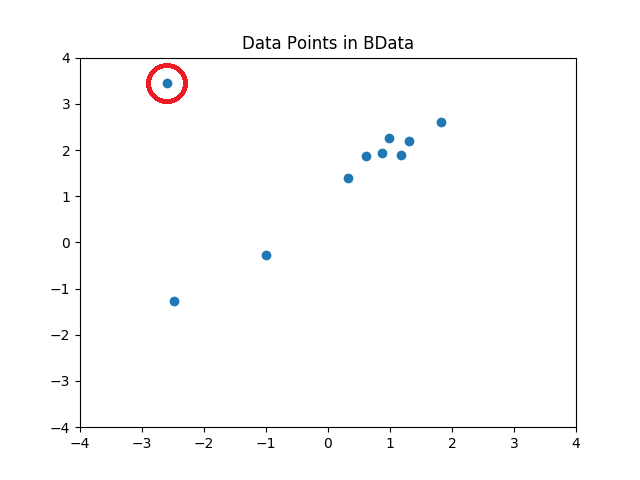
\includegraphics[width=\linewidth]{../P3/figs/B_data.png}
        \end{subfigure}%
  \caption*{Plotting all of the data points. The circled point is the outlier.}
\end{figure}

Two ways to deal with outliers include 1) upper-bounding errors incurred by single points, or 2) removing the points entirely. We experimented with removing the outlier point and ran our ridge regression again.

\begin{center}
 \begin{tabular}{||c c c c||} 
 \hline
 \multicolumn{4}{|c|}{Train on A, Test on Modified B} \\
 \hline
 \hline
 $\lambda$ & Optimal M & Validation MSE & Test MSE\\ [0.5ex] 
 \hline\hline
 0 & 2 & 0.107 & 0.06 \\ 
 \hline
 0.5 & 2 & 0.126 & 0.08 \\
 \hline
 1 & 2 & 0.147 & 0.106 \\
 \hline
 1.5 & 2 & 0.170 & 0.133 \\
 \hline
2 & 1 & 0.188 & 0.158 \\
 \hline
2.5 & 1 & 0.206 & 0.183 \\
 \hline
3 & 1 & 0.225 & 0.209 \\
 \hline
 3.5 & 1 & 0.245 & 0.235 \\
 \hline
4 & 1 & 0.265 & 0.262 \\
 \hline
\end{tabular}
\quad
 \begin{tabular}{||c c c c||} 
 \hline
 \multicolumn{4}{|c|}{Train on Modified B, Test on A} \\
 \hline
 \hline
 $\lambda$ & Optimal M & Validation MSE & Test MSE\\ [0.5ex] 
 \hline\hline
 0 & 3 & 0.089 & 0.193 \\ 
 \hline
 0.5 & 4 & 0.091 & 0.084 \\
 \hline
 1 & 1 & 0.125 & 0.079 \\
 \hline
 1.5 & 1 & 0.132 & 0.077 \\
 \hline
2 & 1 & 0.144 & 0.078 \\
 \hline
2.5 & 1 & 0.159 & 0.084 \\
 \hline
3 & 1 & 0.177 & 0.092 \\
 \hline
 3.5 & 1 & 0.197 & 0.102 \\
 \hline
4 & 1 & 0.218 & 0.115 \\
 \hline
\end{tabular}
\end{center}

We see some differences between the two test runs. When training on A and testing on B, the best model is quadratic, while it is linear when swapping the training and test sets. In both cases, though, the models that performed well had relatively low dimension, which makes sense given what the data looks like. Furthermore, setting $\lambda$ above 3 seemed too harsh of a regularization penalty. Ultimately, given the provided data sets, picking a linear or quadratic model with a small regularization penalty seems like the best bet.

%Insert Table of errors with outlier
%Talk about outlier
%Run again without outlier

%-------------------------------------------
%==============SECTION FOUR=================
%-------------------------------------------

\section{Sparsity and Lasso}

We use the $sklearn$ package in Python to run lasso regression. We run lasso on the training set with different values for the parameter $\lambda$. Next, we test the trained models on the validation set, and find that the model trained with parameter $\lambda = 9.4 \cdot 10^{-4}$ gives the least square loss in the validation set. In particular, we observe that for sufficiently large $\lambda$ $\approx 10^{-3}$, we start to get sparse solutions from lasso, with nonzero coefficients in the second, third, fifth, and sixth terms (which matches those of the true weight vector). Lastly, we test the resulting weights in the test data to check if we overfit.

% (0.46, 0.85) (0.51, 0.74)

In comparison, ridge regression does not give a sparse representation.

See plot below for comparison with ridge regression, ordinary regression with linear basis, and the true function.

\begin{figure}[H]
  \centering
  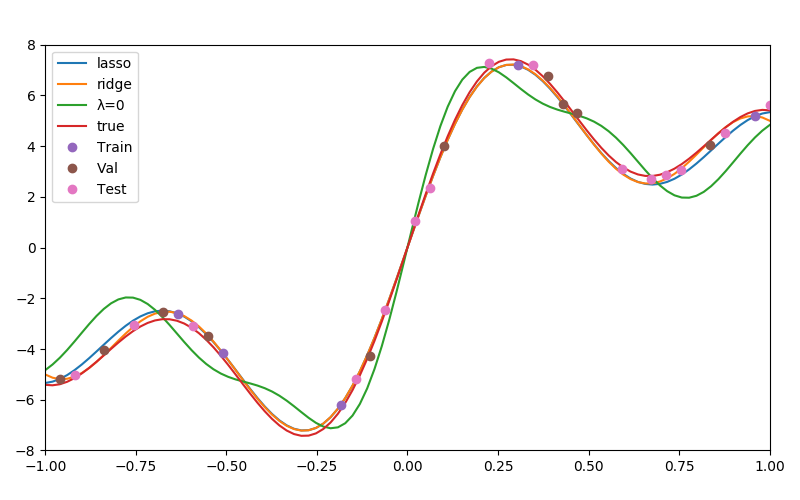
\includegraphics[width = 3in]{../P4/figs/lasso_ridge.png}
  \caption{Lasso vs. Ridge regression}
\end{figure}


% \section{Appendix}
% Coefficients in 2.1

\end{document}